\documentclass[11pt]{article}
\usepackage[a4paper,margin=1in]{geometry}
\usepackage{amsmath,amsfonts}
\usepackage{graphicx}
\usepackage{caption}
\usepackage{enumitem}
\usepackage[hidelinks]{hyperref}
\setlength{\emergencystretch}{8em}
\setlist{nosep}

\title{Valley Regime Study Notes}
\author{}
\date{}

\begin{document}
\sloppy
\maketitle

\section{Model and graph construction (one-way shortcut)}
\begin{itemize}
  \item Nodes are labeled $1,\dots,N$ (paper convention). Internally we use $0,\dots,N-1$.
  \item $K=2k$ neighbors on a ring: each node connects to $\pm 1,\dots,\pm k$ with uniform jump probability $1/K$ (Eq.~1).
  \item Target node is $n=N/2$ (even $N$). Start node $n_0=1$.
  \item Single \textbf{directed} shortcut (paper indexing): $(n_0+5)\to (n+1)$, i.e. $6 \to (N/2+1)$ (one-way, matching the paper).
  \item Internal graph data: padded neighbor table, degrees, directed edge list with weights $1/\deg(\mathrm{src})$.
\end{itemize}

\section{Exact dynamics}
\begin{itemize}
  \item Analytical AW inversion of the generating function is the default solver (max steps fixed to 2000 for stability).
  \item The numerical master-equation iterator is kept only as a validation baseline.
  \item Randomness: MC runs use fixed seeds for reproducibility. Main MC uses seed=0; heatmap storage uses seed+123.
\end{itemize}

\section{Peak and valley detection (Fig.~3 rule)}
\begin{itemize}
  \item Peak at $t$ if $A(t\!-\!1)<A(t)>A(t\!+\!1)$ and $A(t)>10^{-7}$.
  \item If a second peak exists, it must be at least $1\%$ of the highest peak.
  \item For $K=2$ we coarse-grain two steps to suppress parity micro-peaks.
  \item Valley time $t_{\mathrm{valley}}$ is the arg\,min of $A(t)$ between the first two peaks.
\end{itemize}

\section{Monte Carlo (joblib)}
\begin{itemize}
  \item Vectorized batch simulator; batches spawned with independent seeds. Uses \texttt{loky} when allowed; falls back to sequential in restricted environments.
  \item First-passage times are log-binned; density is smoothed with a 7-point moving average for clearer early-time behavior.
\end{itemize}

\section{Classification of trajectories}
\begin{itemize}
  \item Let the first two peaks be at $t_1<t_2$, with valley time $t_{\mathrm{valley}}$ between them, and define $\Delta = \max\{1,\lfloor 0.05 (t_2-t_1)\rfloor\}$.
  \item Classes by first-passage time $T$ (valley + second-peak based split):
  \[
  \begin{aligned}
    \text{direct:}\quad & T < t_{\mathrm{valley}}-\Delta,\\
    \text{valley:}\quad & |T-t_{\mathrm{valley}}|\le \Delta,\\
    \text{intermediate:}\quad & t_{\mathrm{valley}}+\Delta < T \le t_{2}+\Delta,\\
    \text{indirect:}\quad & T > t_{2}+\Delta.
  \end{aligned}
  \]
  \item Note: the usual ``second-peak window'' is $T\in[t_2-\Delta,t_2+\Delta]$, which is contained in the intermediate class.
  \item Heatmaps use full-path MC storage (up to 50k stored paths from a large MC run), split by class.
\end{itemize}

\section{Scan setup}
\begin{itemize}
  \item Even $N\in[10,160]$, $K\in\{2,4,6,8\}$, $\rho=1$.
  \item Bimodality ranges detected under the Fig.~3 rule are printed to stdout.
\end{itemize}

\section{Scan summary (directed shortcut)}
\begin{itemize}
  \item Even $N\in[10,160]$, $K\in\{2,4,6,8\}$, $\rho=1$.
  \item Bimodality detected: $K=2$ none; $K=4$: $N=48..52$; $K=6$: $N=68..104$; $K=8$: $N=14,88..160$.
  \item Explicitly: $K=2$ still shows no two-peak structure under the Fig.~3 rule in this range.
  \item Additional check for $K=2$: with directed shortcut $6\to N/2+1$, coarse-graining by 2 steps (parity fix), and offsets $\{1,2,3,4,5\}$ for even $N\in[6,80]$, no bimodality was found (second peak never reaches the 1\% height criterion).
  \item Visualization: \autoref{fig:bimodality} marks each $(N,K)$ where two peaks exist under the Fig.~3 rule.
\end{itemize}

\begin{figure}[h!]
  \centering
  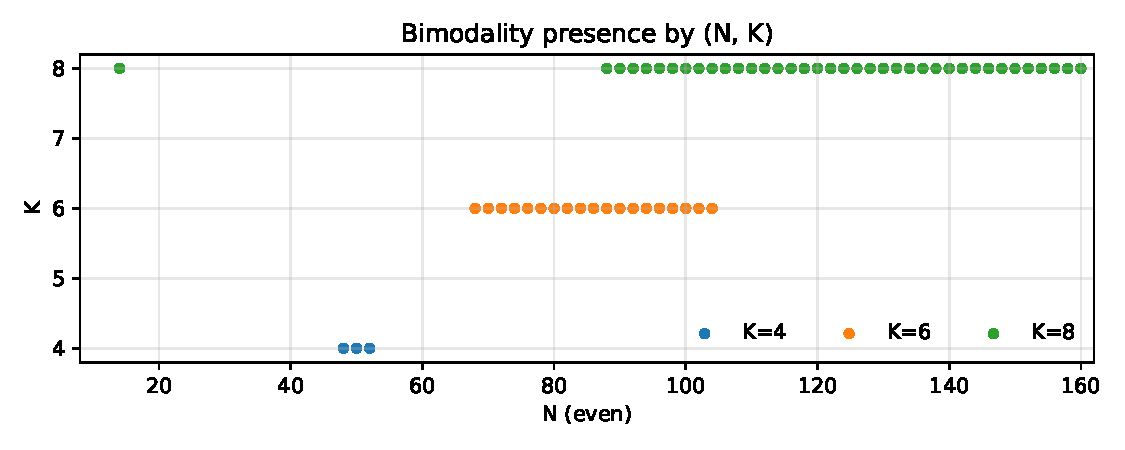
\includegraphics[width=0.78\linewidth]{figures/bimodality_map.pdf}
  \caption{Bimodality map for $K\in\{2,4,6,8\}$, even $N\in[10,160]$.}
  \label{fig:bimodality}
\end{figure}

\section{Single case (N=100, K=6, $\rho=1$)}
\subsection{First-passage distribution}
\begin{figure}[h!]
  \centering
  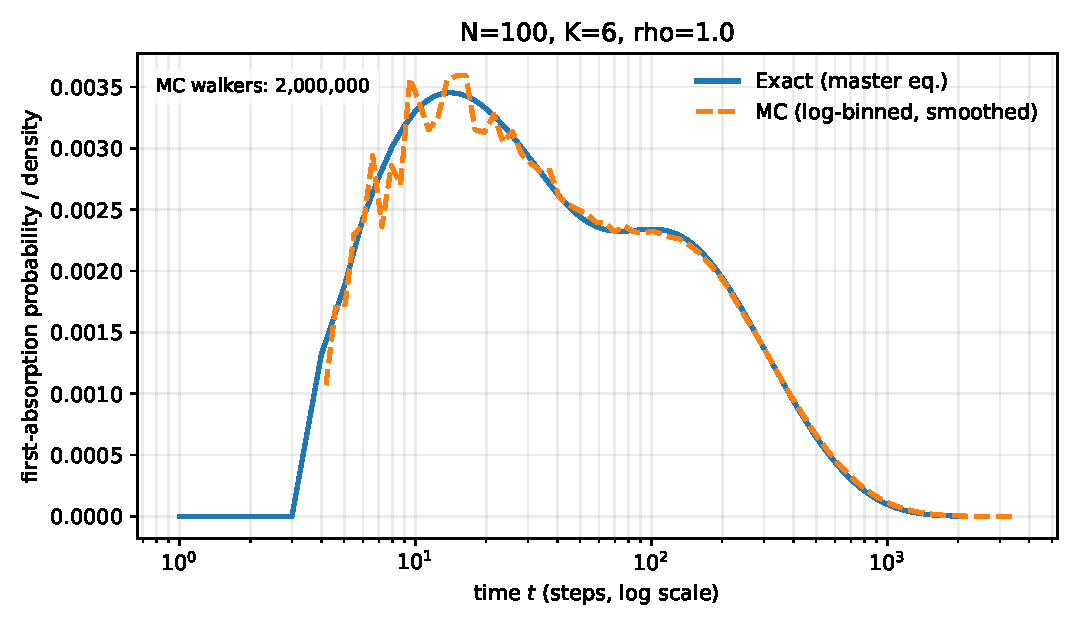
\includegraphics[width=0.8\linewidth]{figures/N100K6_dist.pdf}
  \caption{Exact vs.\ MC first-absorption distribution (MC: log-binned, 7-pt smoothed).}
  \label{fig:dist}
\end{figure}

\subsection{Class definitions and proportions}
\begin{itemize}
  \item Peaks: $t_1=14$, $t_2=101$; valley at $t_{\mathrm{valley}}=74$; $\Delta=4$.
  \item Classes by $T$: direct $<t_{\mathrm{valley}}-\Delta$, valley $|T-t_{\mathrm{valley}}|\le \Delta$, intermediate $t_{\mathrm{valley}}+\Delta < T \le t_2+\Delta$, indirect $>t_2+\Delta$.
  \item MC proportions are shown in \autoref{fig:counts-mc}.
\end{itemize}

\begin{figure}[h!]
  \centering
  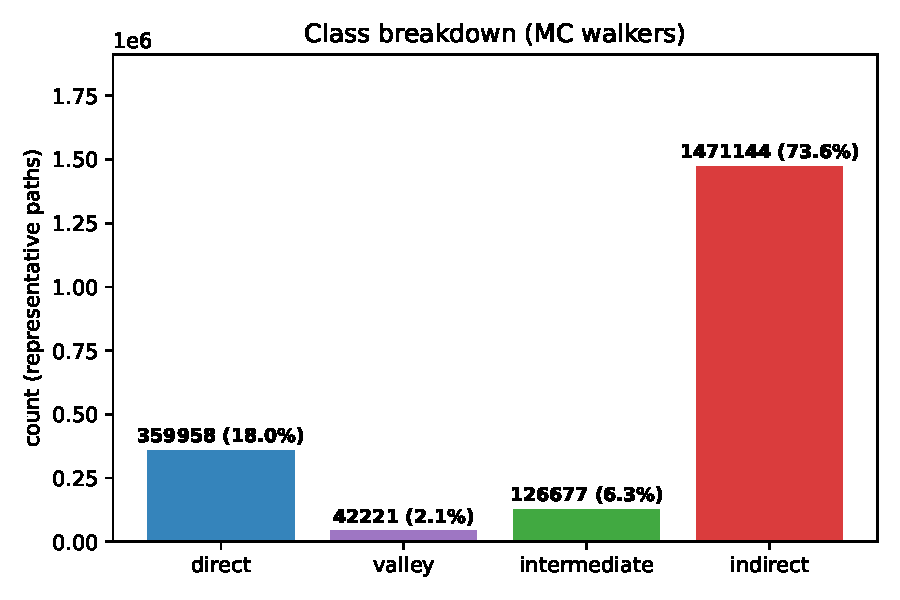
\includegraphics[width=0.55\linewidth]{figures/N100K6_class_counts_mc.pdf}
  \caption{Class breakdown from the MC ensemble.}
  \label{fig:counts-mc}
\end{figure}

\subsection{Shortcut usage (full MC)}
Fractions of walkers using the shortcut edge by class: see \autoref{fig:shortcut}.
Exact fractions are stored in \texttt{data/N100K6\_metrics.json}.

\begin{figure}[h!]
  \centering
  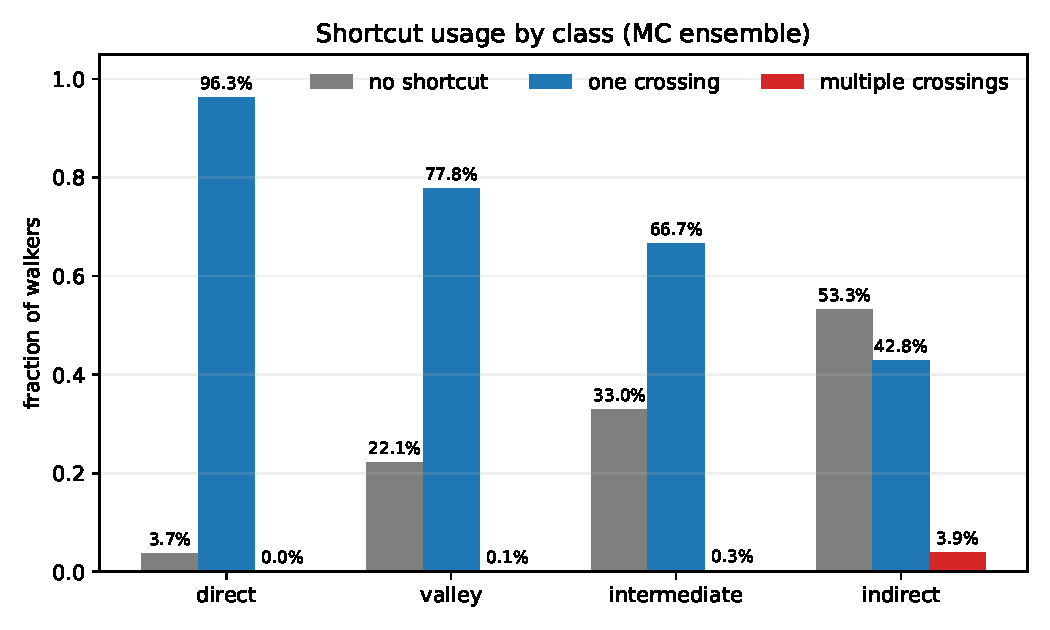
\includegraphics[width=0.75\linewidth]{figures/N100K6_shortcut_usage_mc.pdf}
  \caption{Shortcut usage by class (MC ensemble).}
  \label{fig:shortcut}
\end{figure}

\subsection{Trajectory density heatmaps}
\begin{itemize}
  \item Construction: accumulate visits (time, node) for each class from stored full paths (up to 50k total stored paths from the main MC run, then split by class), per-time normalization to probabilities; Gaussian smoothing ($\sigma=1$); clip at 99th percentile and PowerNorm to highlight weak signals; bilinear interpolation for visual continuity.
  \item Overlays: target line (cyan), shortcut endpoints (gold points at 5\% of the time axis to indicate connectivity).
\end{itemize}

\begin{figure}[h!]
  \centering
  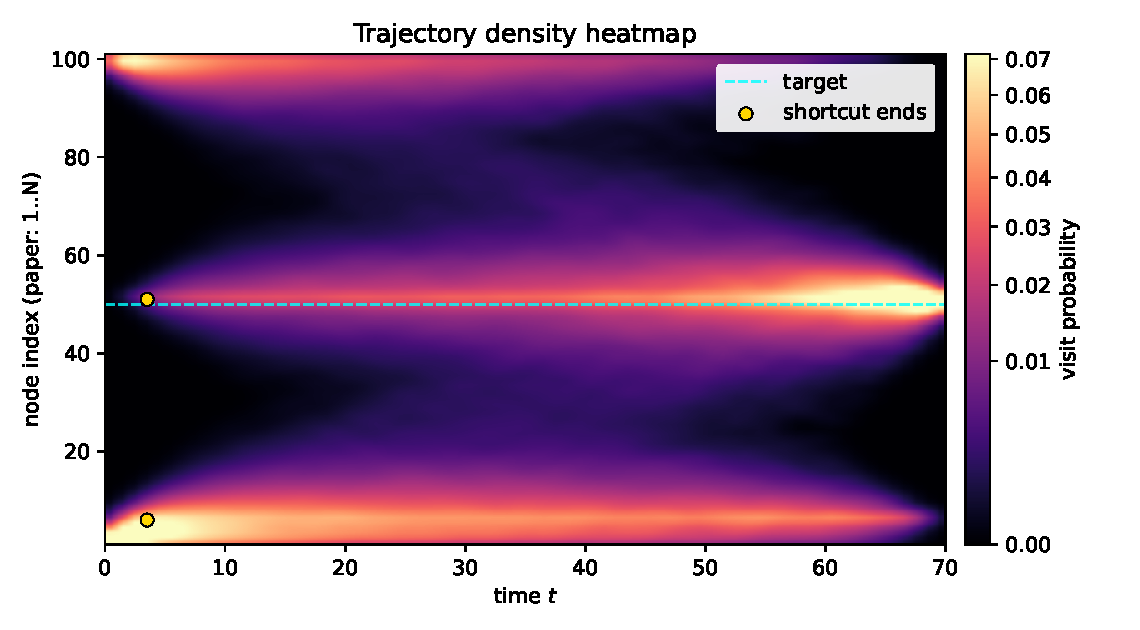
\includegraphics[width=0.8\linewidth]{figures/N100K6_heat_direct.pdf}
  \caption{Heatmap: direct class visit density.}
\end{figure}

\begin{figure}[h!]
  \centering
  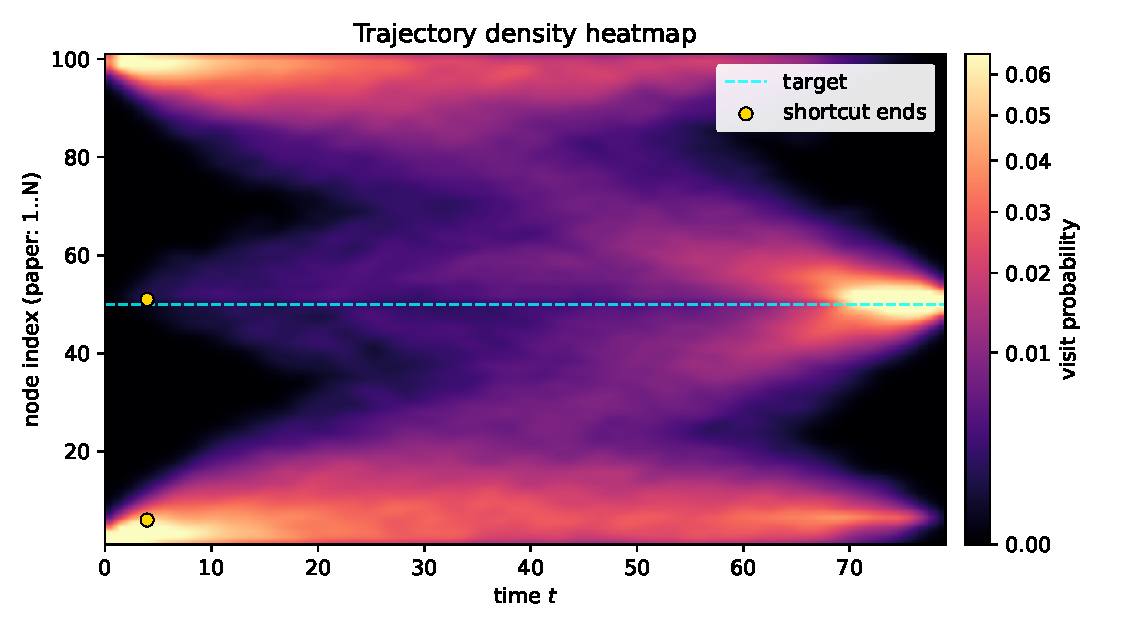
\includegraphics[width=0.8\linewidth]{figures/N100K6_heat_valley.pdf}
  \caption{Heatmap: valley class visit density.}
\end{figure}

\begin{figure}[h!]
  \centering
  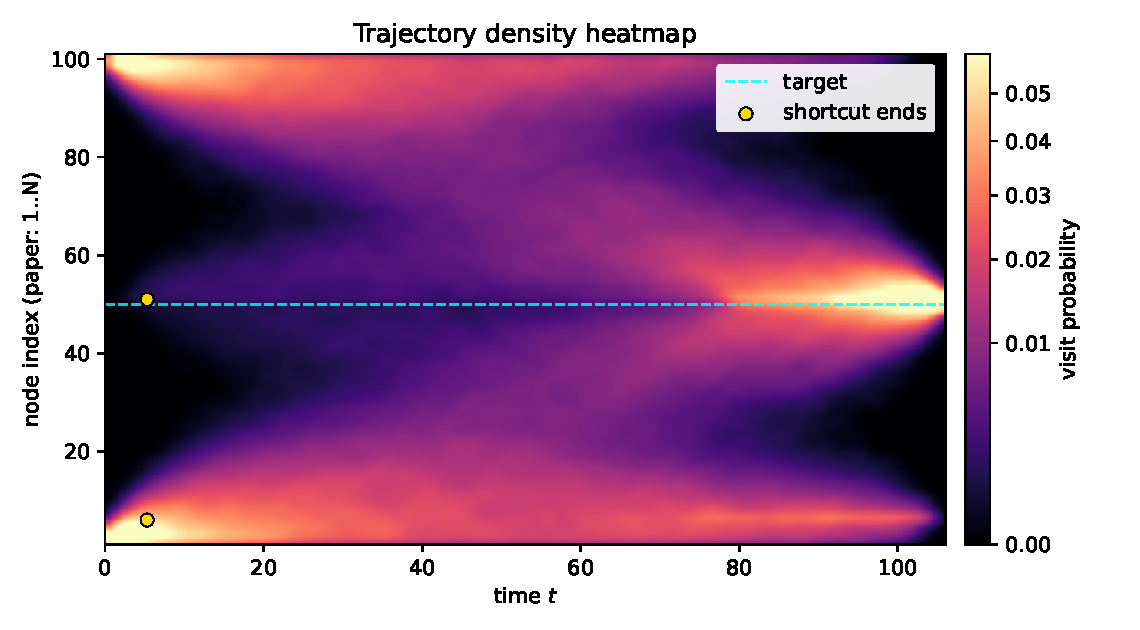
\includegraphics[width=0.8\linewidth]{figures/N100K6_heat_intermediate.pdf}
  \caption{Heatmap: intermediate class visit density.}
\end{figure}

\begin{figure}[h!]
  \centering
  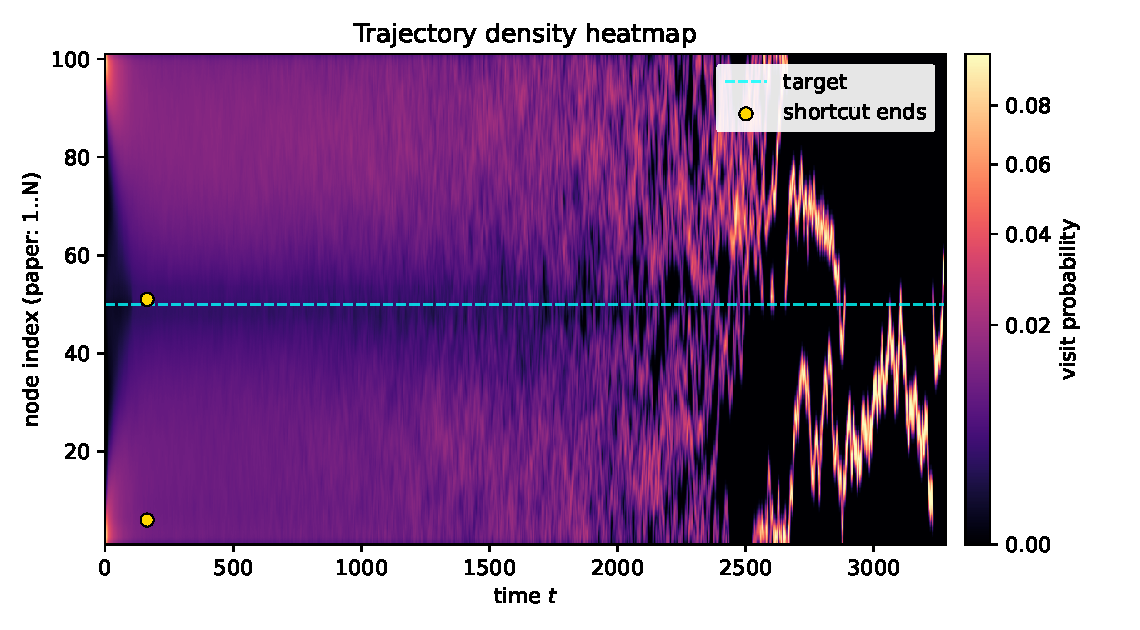
\includegraphics[width=0.8\linewidth]{figures/N100K6_heat_indirect.pdf}
  \caption{Heatmap: indirect class visit density.}
\end{figure}

\section{Data exports and seeds}
\begin{itemize}
  \item Scan raw data: \texttt{data/bimodality\_scan.json} (details for each $K$, $N$, peaks, valley).
  \item Case metrics: \texttt{data/N100K6\_metrics.json} (peaks, valley, $\Delta$, MC class counts, shortcut usage); curves: \texttt{data/N100K6\_curves.npz} (exact $A(t)$ and MC binned density).
  \item Seeds: main MC seed = 0; heatmap storage seed = seed+123; AW max steps = 2000.
\end{itemize}

\section{Data appendix (key values)}
\begin{itemize}
  \item Scan summary (one-way shortcut $6\to N/2+1$, $\rho=1$): $K=2$ none; $K=4$: $N=48..52$; $K=6$: $N=68..104$; $K=8$: $N=14,88..160$. Detailed per-$N$ records in \texttt{data/bimodality\_scan.json}.
  \item N=100, K=6, $\rho=1$: peaks $t_1=14$, $t_2=101$, valley $t_{\mathrm{valley}}=74$, $\Delta=4$ (stored in \texttt{data/N100K6\_metrics.json}).
  \item MC class proportions: see \texttt{figures/N100K6\_class\_counts\_mc.pdf}; shortcut usage fractions stored in \texttt{data/N100K6\_metrics.json}.
  \item Curves: \texttt{data/N100K6\_curves.npz} contains $(t, A_{\text{exact}}(t))$ and MC log-binned density (centers, smoothed density) used in the main distribution plot.
\end{itemize}

\end{document}
